\documentclass[border=10pt]{standalone}

\usepackage[utf8]{inputenc}                                 % Codificação do documento
\usepackage[T1]{fontenc}                                    % Seleção de código de fonte
\usepackage{microtype}                                      % Melhora a justificação do documento
\usepackage{lmodern}                                        % Usa a fonte Latin Modern
\usepackage{ae, aecompl}                                    % Fontes de alta qualidade

\usepackage{amsmath}
\usepackage{verbatim}
\usepackage{tikz}
\usetikzlibrary{arrows,calc,positioning,shadows.blur,decorations.pathreplacing}
\usepackage{etoolbox}

\usepackage{fontawesome}

\begin{document}
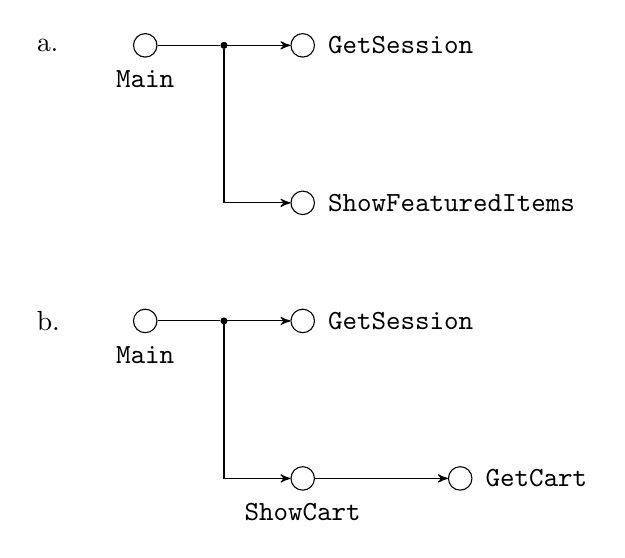
\begin{tikzpicture}
[
	              y = -1cm,
	           ->, >= stealth',
	  node distance = 2cm,
	  vertex/.style = { draw=black, circle, inner sep=3pt },
         dot/.style = { draw=black, fill=black, circle, inner sep=0.75pt },
  coordinate/.style = { draw=none, fill=none, circle, inner sep=0pt, outer sep=0pt },
	   label/.style = { draw=none, fill=none, anchor=west },
	toplabel/.style = { draw=none, fill=none, anchor=north }
]

    \node (1LabelA)                     at (0,0) [label]    {a.};
	
    \node (1MainLabel)                  at (1.5,0.2) [toplabel]    {\texttt{Main}};
    \node (1Main)                       at (1.5,  0) [vertex]      {};

    \node (1MainDot)                    at (2.5,  0) [dot]         {};
    \node (1C1)                         at (2.5,  2) [coordinate]  {};

    \node (1GetSessionLabel)            at (3.7,  0) [label]       {\texttt{GetSession}};
    \node (1GetSession)                 at (3.5,  0) [vertex]      {};
    
    \node (1ShowFeaturedItemsLabel)     at (3.7,  2) [label]       {\texttt{ShowFeaturedItems}};
    \node (1ShowFeaturedItems)          at (3.5,  2) [vertex]      {};

    \draw (1Main) -- (1MainDot) -> (1C1.center) -- (1ShowFeaturedItems);
    \draw (1MainDot) -> (1GetSession);


    \node (2LabelB)              at (  0,3.5) [label]       {b.};
	
    \node (2MainLabel)           at (1.5,3.7) [toplabel]    {\texttt{Main}};
    \node (2Main)                at (1.5,3.5) [vertex]      {};

    \node (2MainDot)             at (2.5,3.5) [dot]         {};
    \node (2C1)                  at (2.5,5.5) [coordinate]  {};

    \node (2GetSessionLabel)     at (3.7,3.5) [label]       {\texttt{GetSession}};
    \node (2GetSession)          at (3.5,3.5) [vertex]      {};
    
    \node (2ShowCartLabel)       at (3.5,5.7) [toplabel]    {\texttt{ShowCart}};
    \node (2ShowCart)            at (3.5,5.5) [vertex]      {};
    \node (2GetCartLabel)        at (5.7,5.5) [label]       {\texttt{GetCart}};
    \node (2GetCart)             at (5.5,5.5) [vertex]      {};

    \draw (2Main) -- (2MainDot) -> (2C1.center) -- (2ShowCart);
    \draw (2MainDot) -> (2GetSession);
    \draw[->] (2ShowCart) edge (2GetCart);

\end{tikzpicture}
\end{document}